\documentclass{beamer}
\usepackage{geometry}
\usepackage[english]{babel}
\usepackage[utf8]{inputenc}
\usepackage{amsmath}
\usepackage{amsfonts}
\usepackage{amssymb}
\usepackage{tikz}
\usepackage{graphicx}
\usepackage{tkz-fct}
\usepackage{venndiagram}

\setlength{\headheight}{26pt}%doesn't seem to fix warning

\usepackage{fancyhdr}
\pagestyle{fancy}
\fancyhf{}

\rhead{\small{5 March 2018}}
\lhead{\small{BECA / Dr. Huson / Mathematics}}

%\vspace{1cm}

\renewcommand{\headrulewidth}{0pt}


\title{Mathematics Class Slides}
\subtitle{Bronx Early College Academy}
\author{Chris Huson}
\date{March 2018}

\begin{document}

\frame{\titlepage}


\section{11.2 Drui}
\frame
{
  \frametitle{GQ: How do we graph polynomials?}
  \framesubtitle{CCSS: HSS.CP.B.6 Understand polynomial functions \qquad \qquad \qquad \alert{11.2}}

  \begin{block}{Do Now: Graph the function $f(x)=x^4-4x^2+3$}
  \begin{enumerate}
    \item What is the degree of the function?\\*[5pt]
    \item What is the sign of its leading coefficient?\\*[5pt]
    \item What is its constant term?\\*[5pt]
  \end{enumerate}
  \end{block}
  Lesson: Features of polynomial functions p. 288\\*[5pt]
  Task: Graph features of polynomials, problem set\\*[5pt]
  Assessment: Graphing problem \#3\\*[5pt]
  Homework: Handout 
}

\frame
{
  \frametitle{Graphing polynomials}
  \framesubtitle{Graph the function $f(x)=x^4-4x^2+3$}
  
    \begin{tikzpicture}[scale=1.0]
      \tkzInit[xmin=-3,xmax=3,ymin=-2,ymax=4]   
      \tkzGrid
      \tkzAxeXY
      \tkzFct[color=blue,thick,domain = -5:5]{x**4-4*x**2+3};
    \end{tikzpicture}

}

\frame
{
  \frametitle{Polynomials}
  \framesubtitle{Each polynomial function can be shown in two forms: standard and factored. \qquad \qquad \qquad \alert{11.2}}
\alert{Standard form}: From largest exponent to smallest\\*
\qquad \alert{Order or degree}: value of the largest exponent\\*
\qquad \alert{Constant term}: the ones value (8, in the example below)
\alert{Factored form}: Product of binomials\\*
\qquad \alert{Factor}: each monomial (e.g. "$(x+1)$)\\*[15pt]
  \begin{enumerate}
    \item Evaluate $f(0)$ and $f(2)$ for each function below.
      \item $f(x)=x^3-5x^2+2x+8$ \qquad \\*[10pt]
      $f(x)=(x+1)(x-2)(x-4)$\\*

  \end{enumerate}
}

\begin{frame}{Vocabulary for polynomial functions}
    Standard form, factored form, order, degree\\*[5pt]
    substitution, long division, remainder\\*[5pt]
    $x$-intercepts, zeros, roots, solutions\\*[5pt]
    $y$-intercept\\*[5pt]
    end behavior, increasing/decreasing, turning points\\*[5pt]
    symmetry, odd/even\\*[5pt]
\end{frame}

\frame
{
  \frametitle{Interpreting a displacement vs time graph}
  \framesubtitle{CCSS: F.IF.B.6 Calculate \& interpret the rate of change of a function}

  \begin{block}{Consider the function $f(x)=-x^2+2x+3$}
  \begin{enumerate}
      \item Factor $f$ and state its zeros.
      \item Restate $f$ in vertex form. Write down the vertex as an ordered pair.
      \item Over what intervals is the function increasing, decreasing, and neither?
      \item If $f(x)$ represents the height of a diver over the domain $0 \leq x \leq 3$, interpret $f(0)$, the vertex, and $f(3)$
      \item What does the "slope" of the curve represent?
  \end{enumerate}
  \end{block}
}


\end{document}
